% ¿De dónde sale el agua del mapa? Paso a paso (Beamer 16:9).
% Figuras: python herramientas/figuras/figuras_agua.py  ·  Compilar dos veces: pdflatex presentacion_agua_paso_a_paso.tex
\documentclass[aspectratio=169,11pt]{beamer}
\usepackage[utf8]{inputenc}
\usepackage[T1]{fontenc}
\IfFileExists{spanish.ldf}{\usepackage[spanish,es-noshorthands]{babel}}{}
\usepackage{lmodern}
\usepackage{booktabs}
\usepackage{tabularx}
\usepackage{array}
\usepackage{tikz}
\usetikzlibrary{arrows.meta,positioning}
\graphicspath{{figuras/}}

% ---------- estilo (el mismo de presentacion_avance.tex) ----------
\definecolor{azul}{HTML}{0B3D5C}
\definecolor{azulc}{HTML}{0B5D8F}
\definecolor{celeste}{HTML}{9FD3F2}
\definecolor{acento}{HTML}{D4145A}
\definecolor{ok}{HTML}{1B7F4B}
\definecolor{naranja}{HTML}{E8710A}
\definecolor{gris}{HTML}{5B6770}
\usetheme{default}
\setbeamercolor{frametitle}{fg=white,bg=azul}
\setbeamercolor{structure}{fg=azulc}
\setbeamercolor{alerted text}{fg=acento}
\setbeamercolor{block title}{fg=white,bg=azulc}
\setbeamercolor{block body}{bg=azulc!7}
\setbeamercolor{block title alerted}{fg=white,bg=acento}
\setbeamercolor{block body alerted}{bg=acento!7}
\setbeamercolor{block title example}{fg=white,bg=ok}
\setbeamercolor{block body example}{bg=ok!7}
\setbeamertemplate{navigation symbols}{}
\setbeamertemplate{itemize items}[circle]
\setbeamerfont{frametitle}{size=\large,series=\bfseries}
\setbeamertemplate{frametitle}{\nointerlineskip\begin{beamercolorbox}[wd=\paperwidth,ht=2.6ex,dp=1.3ex,leftskip=1em]{frametitle}\insertframetitle\end{beamercolorbox}}
\setbeamertemplate{footline}{\hbox{\begin{beamercolorbox}[wd=\paperwidth,ht=2.4ex,dp=1ex,leftskip=1em,rightskip=1em]{}%
  \color{gris}\tiny ¿De dónde sale el agua del mapa? · Tumbes y Piura · PEU-CD INEI\hfill\insertframenumber/\inserttotalframenumber\end{beamercolorbox}}}
\tikzset{caja/.style={draw=azulc,fill=azulc!8,rounded corners=2pt,align=center,font=\scriptsize,minimum height=1.25cm,text width=2.1cm,inner sep=2pt},
         flecha/.style={-{Stealth[length=2.2mm]},thick,azulc}}

\begin{document}

% ---------- portada ----------
{\setbeamertemplate{footline}{}
\begin{frame}
\begin{tikzpicture}[remember picture,overlay]
  \fill[azul] (current page.north west) rectangle ([yshift=-5.3cm]current page.north east);
  \node[anchor=north west,text width=13.5cm,text=white] at ([xshift=1cm,yshift=-1.1cm]current page.north west)
    {{\LARGE\bfseries ¿Cómo sabemos que esa área tiene agua?}\\[8pt]
     {\large De la imagen de satélite al polígono azul del mapa, paso a paso}};
  \node[anchor=north west,text width=13.5cm] at ([xshift=1cm,yshift=-6.0cm]current page.north west)
    {\large Christopher · Maykol · Marcia · Luz Ángela\\[4pt]
     \normalsize Proyecto integrador PEU Ciencia de Datos (INEI) · noviembre de 2026\\[10pt]
     \small\color{gris} Código: \texttt{src/huellas.py}, \texttt{src/impacto.py}, \texttt{src/validar\_radar.py}, \texttt{herramientas/figuras\_agua.py}};
\end{tikzpicture}
\end{frame}}

% ---------- 1 ----------
\begin{frame}{Dos fuentes distintas pintan agua en el mapa}
\begin{columns}[T]
\column{0.48\textwidth}
\begin{block}{Radar Sentinel-1: lo que se observó}
\small
\begin{itemize}
\item Satélite de la Agencia Espacial Europea (programa Copernicus).
\item Detecta agua \alert{nueva} comparando el evento con la temporada seca.
\item Capas: 2017 (feb--abr), 2023 (mar--abr) y últimos 24 días.
\item Es un \alert{mínimo}: no ve agua entre casas ni bajo árboles.
\end{itemize}
\end{block}
\column{0.48\textwidth}
\begin{block}{JRC: lo que podría inundarse}
\small
\begin{itemize}
\item Mapa del Centro Común de Investigación de la Comisión Europea (CEMS-GloFAS v2, 90 m).
\item Sale de un \alert{modelo} hidrológico e hidráulico, no de una foto.
\item Escenarios: crecida de 1 en 10 y de 1 en 100 años, con profundidad.
\item No es un pronóstico: no dice que pasará este año.
\end{itemize}
\end{block}
\end{columns}
\vspace{6pt}
\centering\small Las dos se cruzan con la misma población (WorldPop) y edificaciones (Google Open Buildings).
\end{frame}

% ---------- 2 ----------
\begin{frame}{El camino completo del radar}
\centering
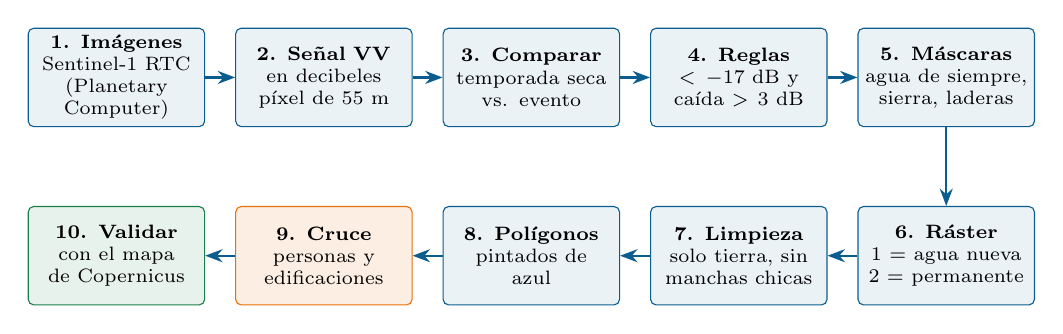
\begin{tikzpicture}[node distance=0.38cm]
\node[caja] (a) {\textbf{1. Imágenes}\\Sentinel-1 RTC\\(Planetary Computer)};
\node[caja,right=of a] (b) {\textbf{2. Señal VV}\\en decibeles\\píxel de 55 m};
\node[caja,right=of b] (c) {\textbf{3. Comparar}\\temporada seca\\vs. evento};
\node[caja,right=of c] (d) {\textbf{4. Reglas}\\$<-17$ dB y\\caída $>3$ dB};
\node[caja,right=of d] (e) {\textbf{5. Máscaras}\\agua de siempre,\\sierra, laderas};
\node[caja,below=1.0cm of e] (f) {\textbf{6. Ráster}\\1 = agua nueva\\2 = permanente};
\node[caja,left=of f] (g) {\textbf{7. Limpieza}\\solo tierra, sin\\manchas chicas};
\node[caja,left=of g] (h) {\textbf{8. Polígonos}\\pintados de\\azul};
\node[caja,left=of h,fill=naranja!12,draw=naranja] (i) {\textbf{9. Cruce}\\personas y\\edificaciones};
\node[caja,left=of i,fill=ok!10,draw=ok] (j) {\textbf{10. Validar}\\con el mapa\\de Copernicus};
\draw[flecha] (a)--(b); \draw[flecha] (b)--(c); \draw[flecha] (c)--(d); \draw[flecha] (d)--(e);
\draw[flecha] (e)--(f); \draw[flecha] (f)--(g); \draw[flecha] (g)--(h); \draw[flecha] (h)--(i); \draw[flecha] (i)--(j);
\end{tikzpicture}
\vspace{8pt}

\small Ejemplos: \textbf{Bajo Piura, El Niño costero de 2017} (ventana de 42 $\times$ 45 km),\\
donde Copernicus hizo un mapa oficial de la inundación (activación EMSR199).
\end{frame}

% ---------- 3 ----------
\begin{frame}{Paso 1--2: qué mide el radar}
\begin{columns}[T]
\column{0.55\textwidth}
\small
\begin{itemize}\setlength\itemsep{4pt}
\item El satélite \textbf{emite} microondas y mide cuánto \textbf{rebota} hacia él (retrodispersión, en dB).
\item Atraviesa las nubes y funciona de noche: sirve justo cuando llueve.
\item Pasa sobre Tumbes y Piura cada pocos días (14 pasadas entre el 12/10 y el 3/11/2026).
\item Usamos la polarización \textbf{VV} y promediamos 3 $\times$ 3 píxeles para reducir el ruido (moteado).
\end{itemize}
\column{0.42\textwidth}
\begin{block}{La idea clave}
\small
\textbf{Agua calma = espejo.} La señal rebota lejos del satélite y vuelve muy poca: el píxel se ve \textbf{oscuro} (VV muy negativo).\\[4pt]
Suelo, cultivos y casas son rugosos: devuelven más señal y se ven claros.
\end{block}
\end{columns}
\end{frame}

% ---------- 4 ----------
\begin{frame}{Paso 3: comparar la temporada seca con el evento}
\centering
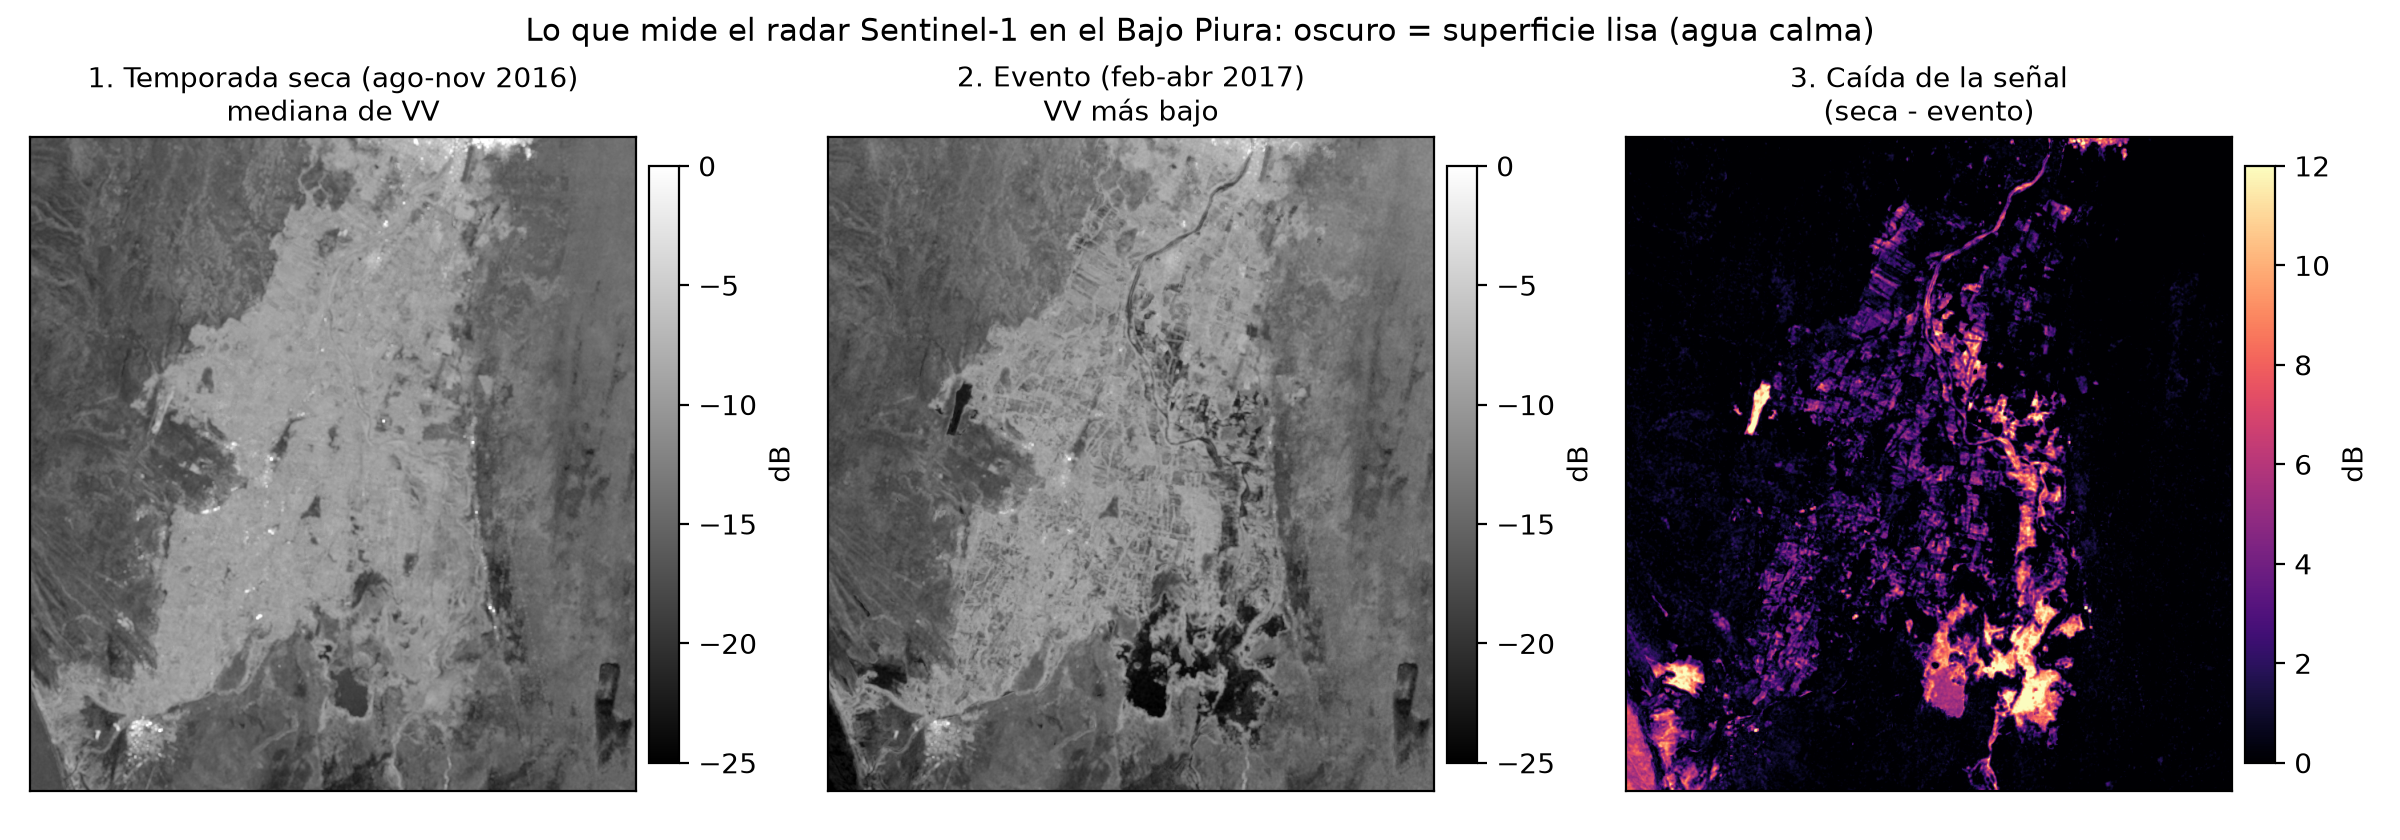
\includegraphics[width=\textwidth]{agua_1_radar.png}\\[2pt]
\small \textbf{Seca:} mediana de 9 pasadas (ago--nov 2016). \textbf{Evento:} el valor más bajo de 13 pasadas (feb--abr 2017).\\
Lo que se oscureció mucho (derecha, colores claros) es candidato a agua nueva.
\end{frame}

% ---------- 5 ----------
\begin{frame}{Un píxel en el tiempo}
\centering
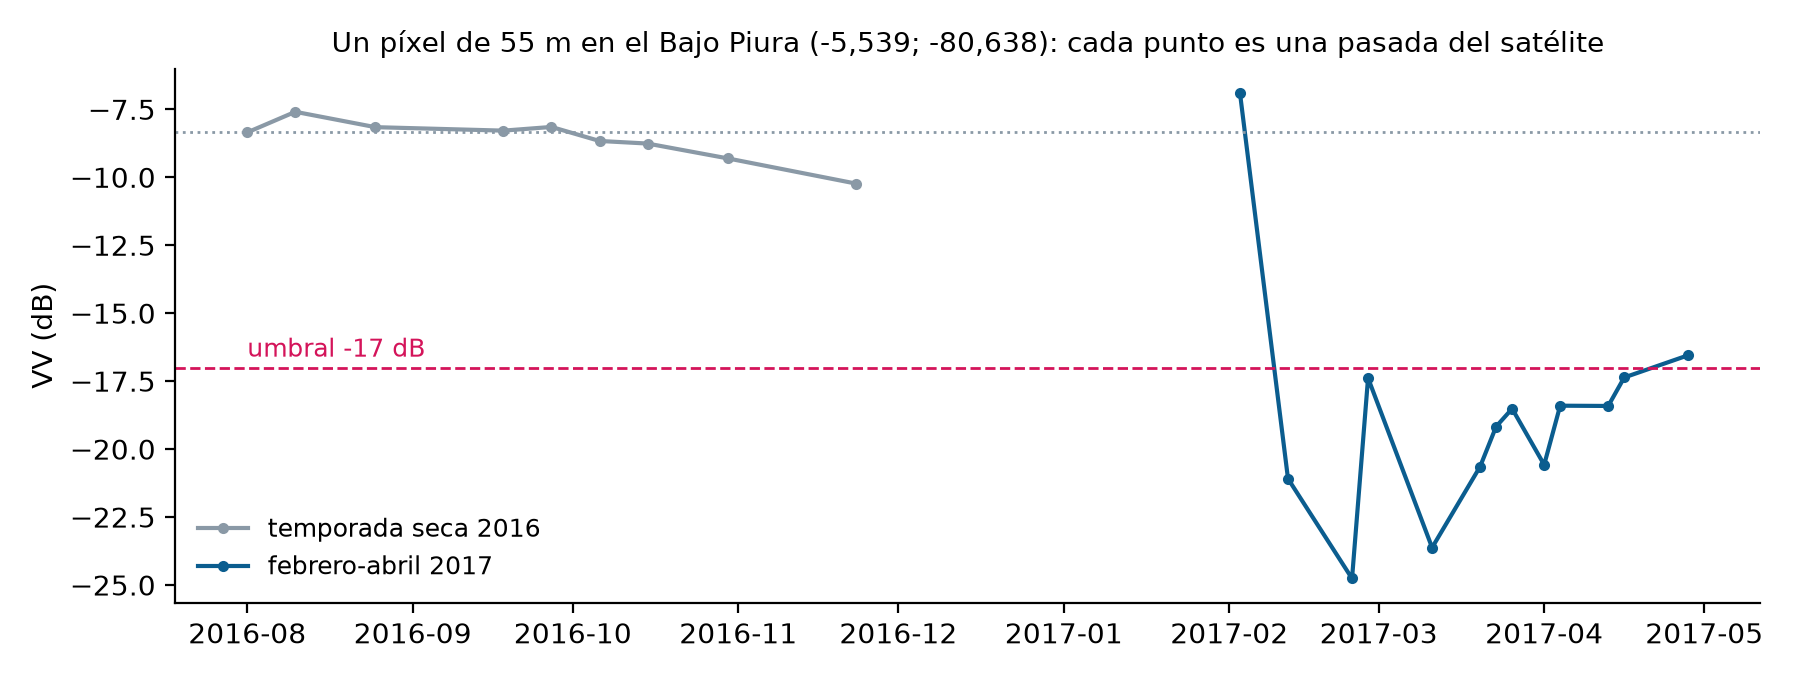
\includegraphics[width=0.92\textwidth]{agua_2_pixel.png}\\[2pt]
\small En la temporada seca el píxel estaba cerca de \textbf{$-$8,3 dB}. En marzo de 2017 bajó hasta \textbf{$-$24,8 dB}:\\
cruzó el umbral y cayó 16,5 dB. Por eso se marca como agua.
\end{frame}

% ---------- 6 ----------
\begin{frame}{Paso 4: ¿por qué $-$17 dB?}
\begin{columns}[c]
\column{0.55\textwidth}
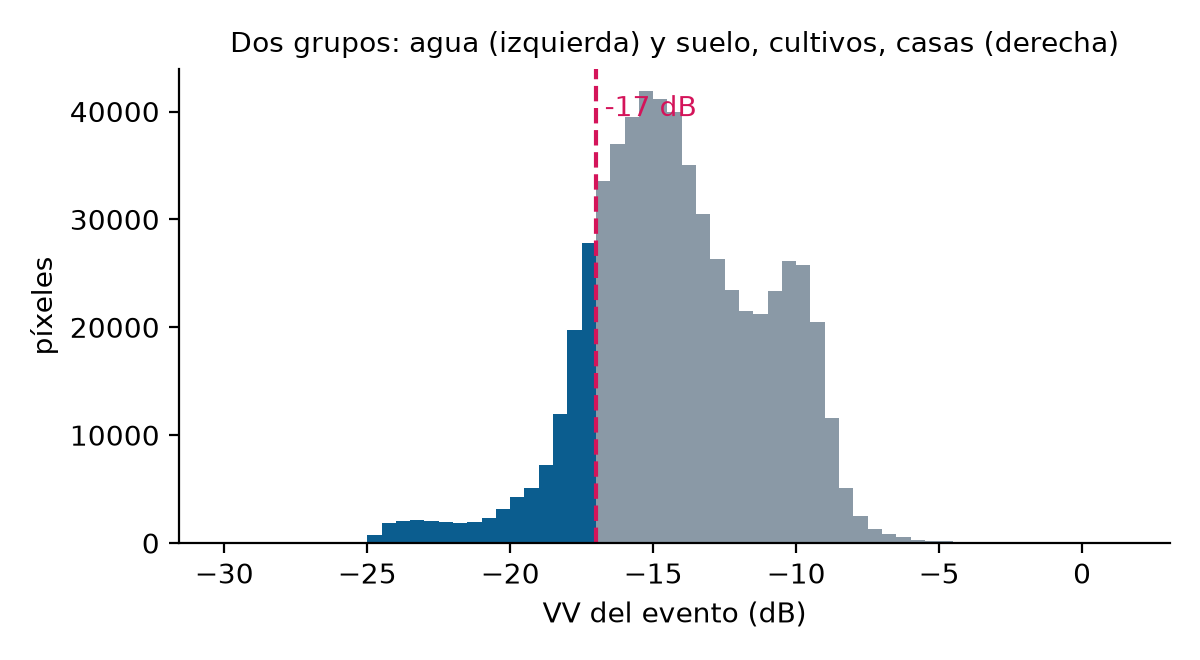
\includegraphics[width=\textwidth]{agua_4_histograma.png}
\column{0.43\textwidth}
\small
\begin{itemize}\setlength\itemsep{4pt}
\item Los valores forman dos grupos: agua (izquierda) y todo lo demás.
\item $-$17 dB está entre los dos, como en la literatura (Twele et al., 2016).
\item El umbral automático de Otsu (1979) en los últimos 24 días dio $-$16,8 dB: casi el mismo.
\item Además pedimos que la señal \textbf{baje más de 3 dB} frente a la temporada seca: así no se cuenta lo que ya era oscuro (arena lisa, salinas).
\end{itemize}
\end{columns}
\end{frame}

% ---------- 7 ----------
\begin{frame}{Pasos 4--5: cada regla quita falsos positivos}
\centering
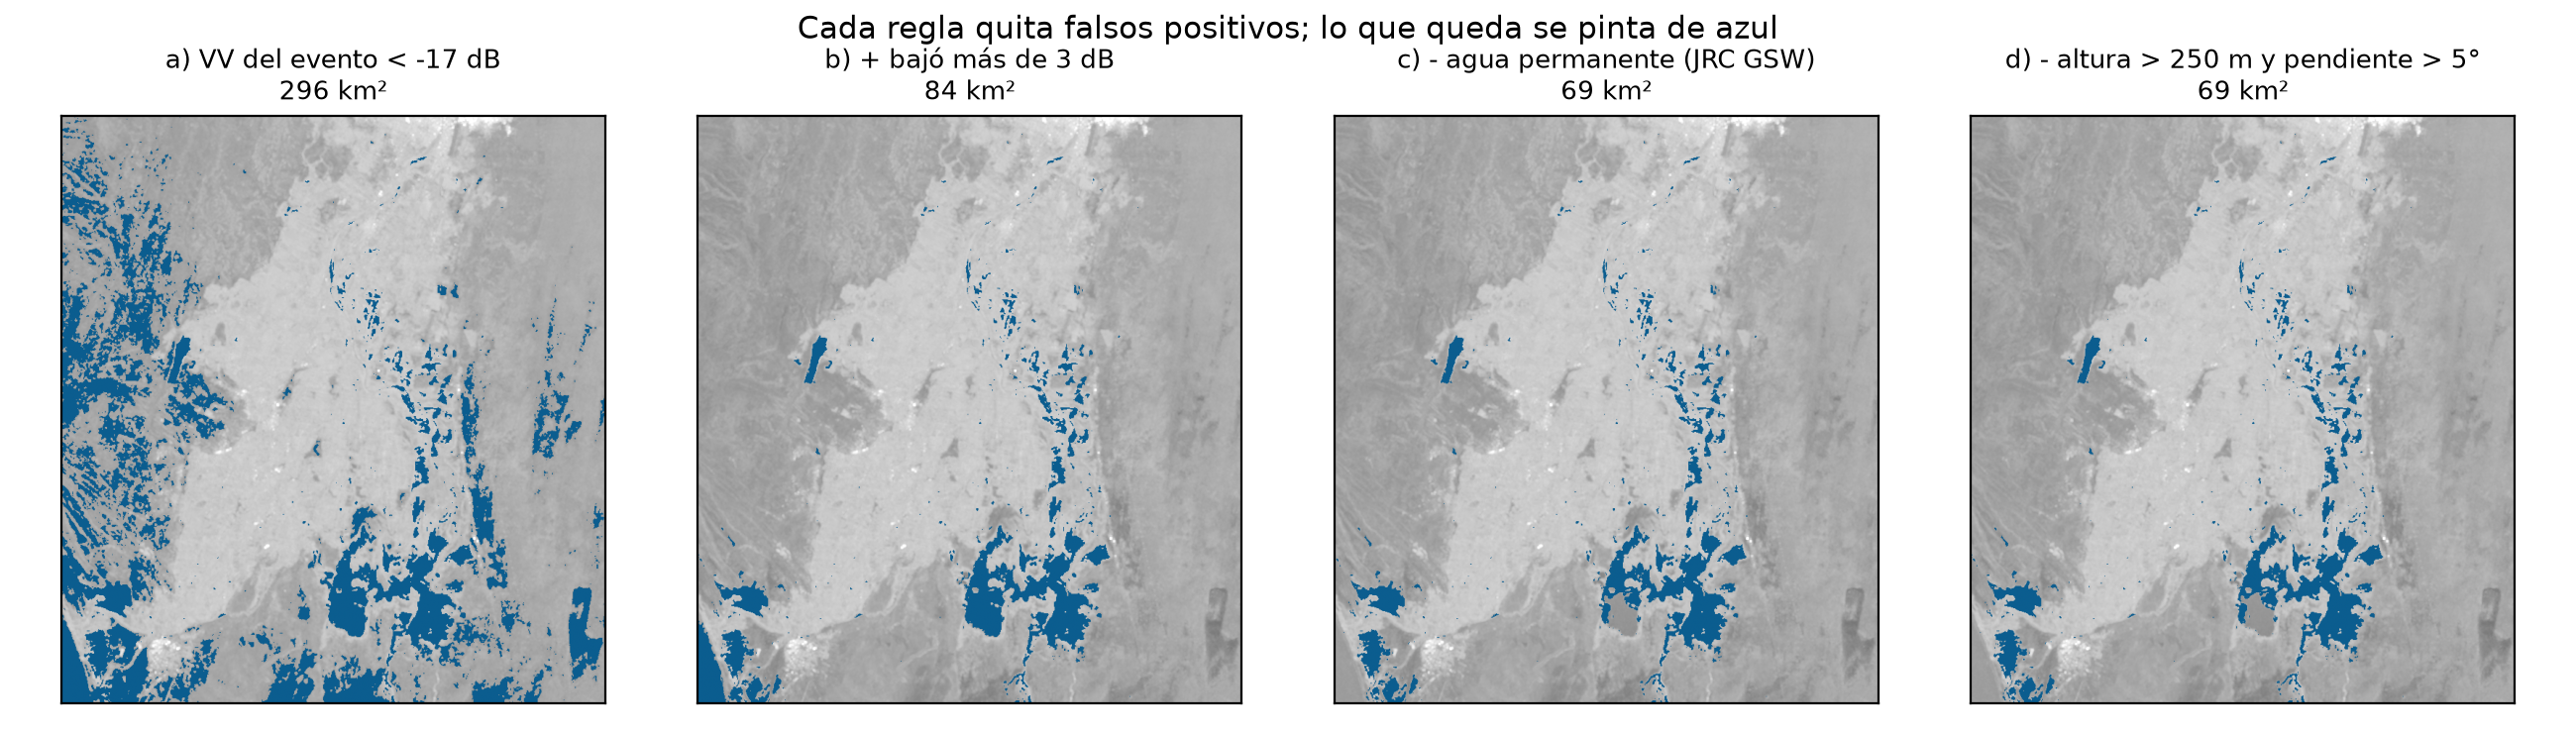
\includegraphics[width=\textwidth]{agua_3_reglas.png}\\[2pt]
\footnotesize\setlength{\tabcolsep}{5pt}
\begin{tabular}{@{}lcccc@{}}
\toprule
 & a) $<-17$ dB & b) + caída $>3$ dB & c) sin agua permanente & d) sin sierra ni pendiente\\
\midrule
km² & 296 & 84 & 69 & 69\\
\bottomrule
\end{tabular}\\[3pt]
\footnotesize Agua permanente: JRC Global Surface Water (agua presente $\geq$ 75 \% del tiempo, 1984--2021). Altura $>$ 250 m o pendiente $>$ 5°: Copernicus DEM 30 m (en esta ventana plana no quita nada).
\end{frame}

% ---------- 8 ----------
\begin{frame}{Pasos 6--8: del ráster al polígono azul}
\begin{columns}[T]
\column{0.52\textwidth}
\small
\begin{enumerate}\setlength\itemsep{4pt}
\item[6.] Se guarda un ráster de 55 m: \textbf{1} = agua nueva, \textbf{2} = agua permanente (\texttt{data/huellas/2017.tif}).
\item[7.] Se deja solo la tierra de los 76 distritos y se borran manchas menores de 0,03 km².
\item[8.] El ráster se convierte en polígonos (\texttt{impacto.poligonos()}) y el tablero los pinta:
  \begin{itemize}
  \item \textcolor{celeste!70!black}{\textbf{celeste}}: el río de siempre;
  \item \textcolor{azulc}{\textbf{azul}}: agua nueva del evento.
  \end{itemize}
\end{enumerate}
\column{0.45\textwidth}
\begin{alertblock}{Por qué se ve tosco al acercarse}
\small Para que el archivo sea liviano, los píxeles se agrupan de 2 en 2 (unos 110 m) y los bordes se simplifican. Es una tarea pendiente: dibujar a 55 m.
\end{alertblock}
\end{columns}
\end{frame}

% ---------- 9 ----------
\begin{frame}{Qué es el mapa de JRC}
\begin{columns}[T]
\column{0.5\textwidth}
\small
\begin{itemize}\setlength\itemsep{4pt}
\item Producto del servicio de emergencias Copernicus (CEMS) y GloFAS (Dottori et al., 2016).
\item Un modelo hidrológico calcula el caudal de una crecida rara (la que ocurre en promedio 1 vez cada 10 o 100 años).
\item Un modelo hidráulico reparte esa agua sobre el relieve y da la \textbf{profundidad} en cada celda de 90 m.
\item Lo recortamos a los distritos de Tumbes y Piura.
\end{itemize}
\column{0.46\textwidth}
\begin{alertblock}{Límites}
\small
\begin{itemize}
\item Solo ríos grandes: no modela quebradas ni lluvia que se empoza en la ciudad.
\item No tiene en cuenta defensas ribereñas ni obras recientes.
\item Es un escenario: no dice cuándo pasará.
\end{itemize}
\end{alertblock}
\end{columns}
\end{frame}

% ---------- 10 ----------
\begin{frame}{Paso 10: ¿funciona? Comparación con el mapa oficial de 2017}
\begin{columns}[c]
\column{0.62\textwidth}
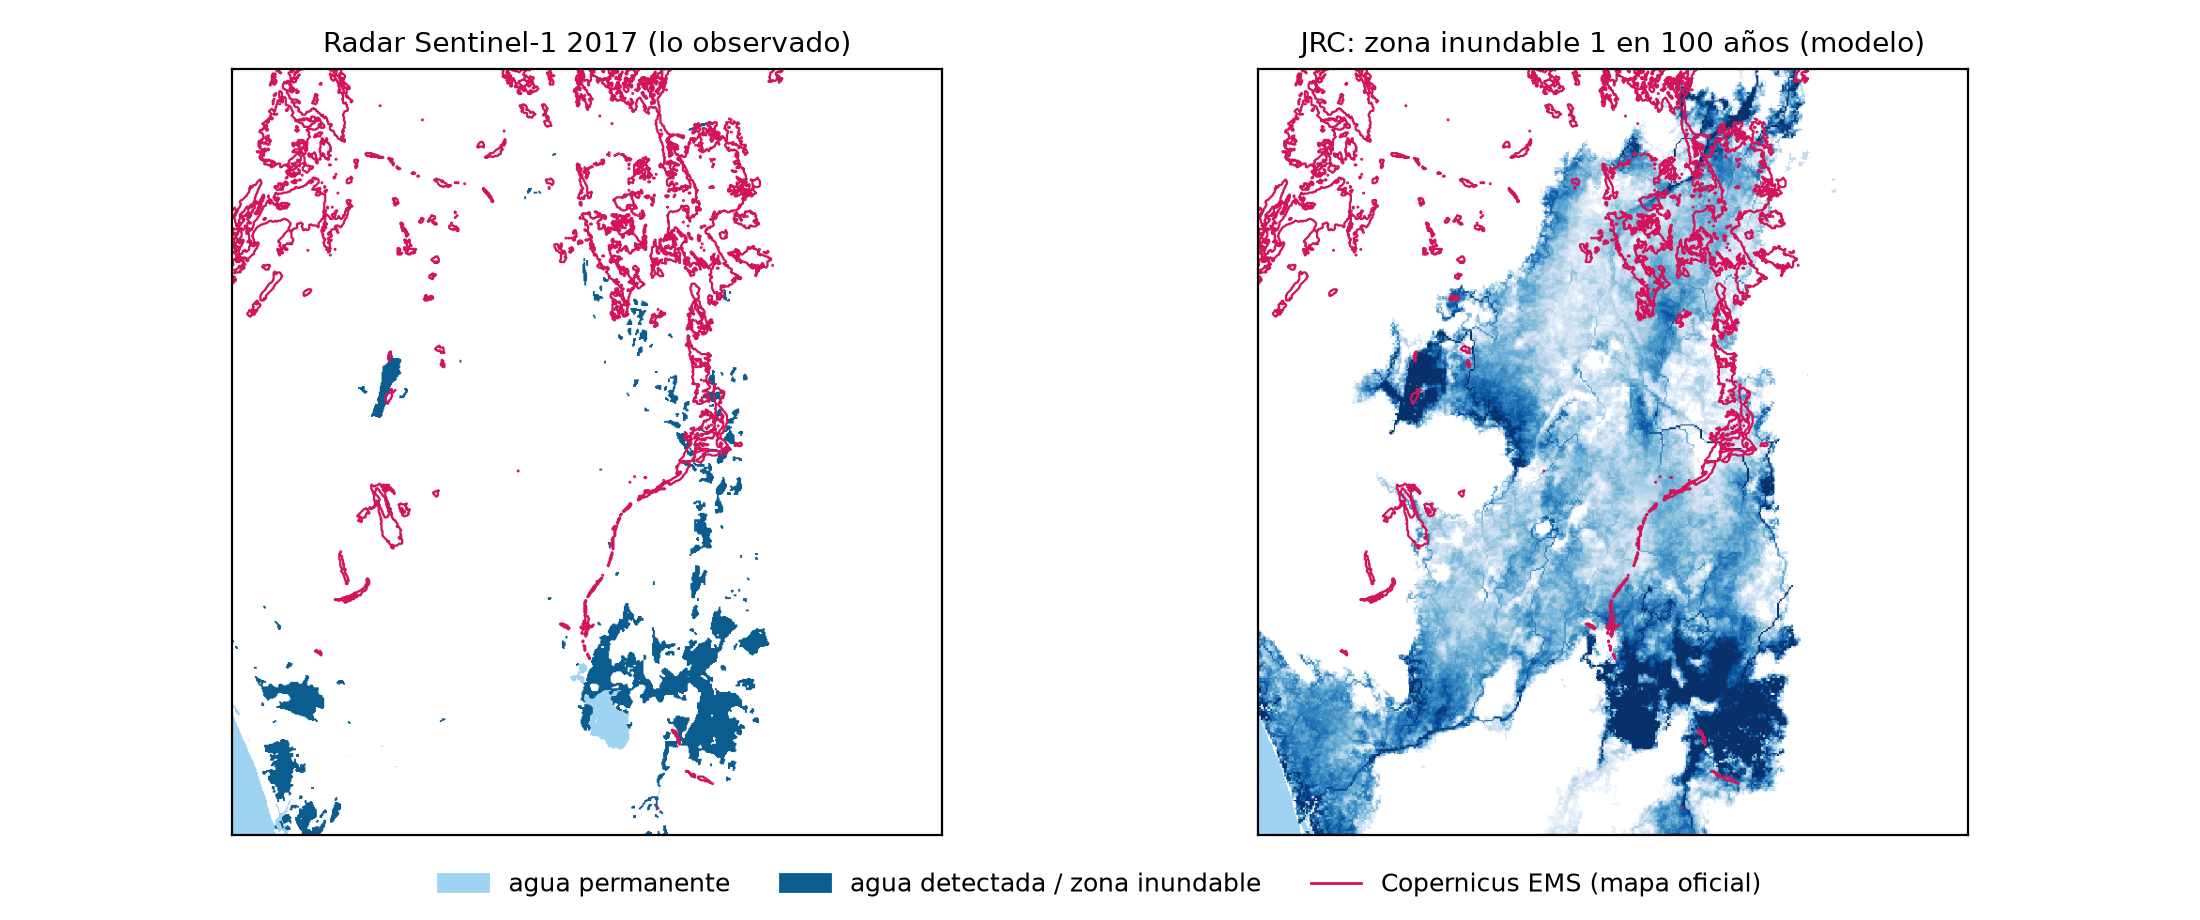
\includegraphics[width=\textwidth]{agua_5_comparacion.png}
\column{0.36\textwidth}
\footnotesize\setlength{\tabcolsep}{4pt}
\begin{tabular}{@{}lcc@{}}
\toprule
4 áreas de Piura & Radar & JRC\\
\midrule
Acierto & 42 \% & 85 \%\\
Precisión & 63 \% & 32 \%\\
\bottomrule
\end{tabular}\\[2pt]
\scriptsize Acierto: parte del área oficial que se detecta. Precisión: parte de lo marcado que es agua oficial.\\[5pt]
\footnotesize
\textbf{Radar:} lo que marca casi siempre es agua, pero se le escapa más de la mitad.\\[3pt]
\textbf{JRC:} cubre casi todo lo que se inundó, pero marca un área mucho mayor.\\[3pt]
\scriptsize Mapa oficial: imágenes Cosmo-SkyMed y Radarsat, 23 al 30/3/2017 (\texttt{validacion\_2017.json}).
\end{columns}
\end{frame}

% ---------- 11 ----------
\begin{frame}{Paso 9: cruce con edificaciones y personas}
\centering
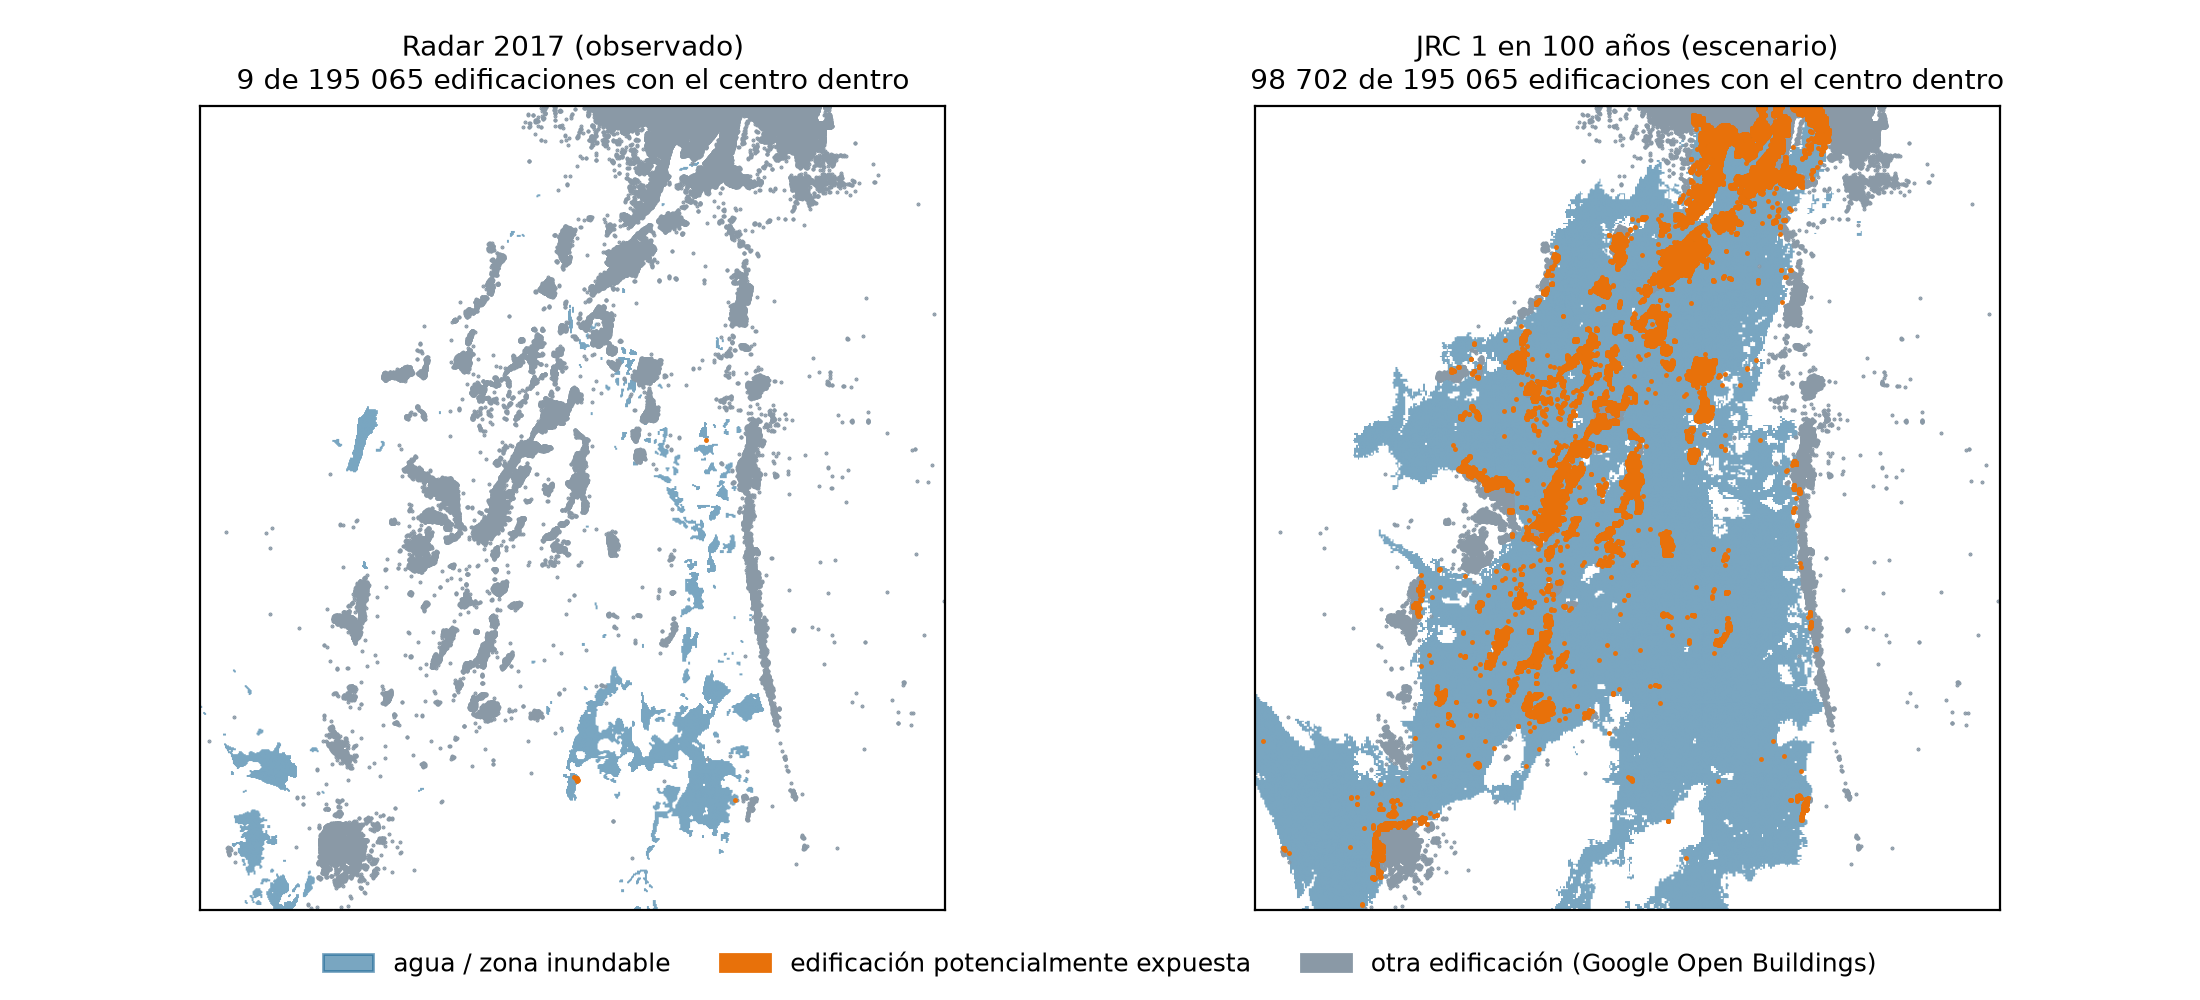
\includegraphics[width=0.78\textwidth]{agua_6_cruce.png}\\
\small \textbf{Edificación expuesta} = su centro cae dentro del agua (Google Open Buildings v3, no son viviendas censales).\\
\textbf{Población expuesta} = población WorldPop de cada celda de 100 m $\times$ fracción de la celda con agua.
\end{frame}

% ---------- 12 ----------
\begin{frame}{Lo que el radar no ve (y por qué el tablero puede no mostrar una noticia)}
\begin{columns}[T]
\column{0.5\textwidth}
\small
\begin{itemize}\setlength\itemsep{4pt}
\item \textbf{Ciudades:} paredes y agua forman un rebote doble que \emph{aumenta} la señal. En la ventana, el radar marca agua en 9 de 195~065 edificaciones; el mapa oficial de Copernicus, en 27.
\item \textbf{Lluvia sobre la ciudad} (calles anegadas, techos): no es desborde. En Piura, INDECI cuenta 997~173 afectados por lluvia intensa y 130~482 por inundación (2003--2024).
\item \textbf{Sierra:} se excluye lo que está a más de 250 m o con pendiente mayor de 5°.
\item \textbf{Inundaciones de pocas horas} que pasan entre dos pasadas del satélite.
\end{itemize}
\column{0.46\textwidth}
\begin{block}{Cómo lo usamos entonces}
\small
\begin{itemize}
\item Radar = \textbf{mínimo observado} fuera de las ciudades.
\item JRC = \textbf{zona donde puede llegar} el agua: de ahí salen las cifras principales (399~506 personas en la zona 1/100).
\item El tablero no emite alertas: las oficiales son de SENAMHI, ENFEN e INDECI.
\end{itemize}
\end{block}
\end{columns}
\end{frame}

% ---------- 13 ----------
\begin{frame}{Prueba con noticias (11/10 al 4/11/2026)}
\scriptsize
\renewcommand{\arraystretch}{1.15}
\begin{tabularx}{\textwidth}{@{}>{\raggedright\arraybackslash}p{2.9cm} >{\raggedright\arraybackslash}p{3.6cm} c >{\raggedright\arraybackslash}X@{}}
\toprule
\textbf{Lugar} & \textbf{Noticia} & \textbf{Agua detectada} & \textbf{Por qué}\\
\midrule
Aguas Verdes (Zarumilla) & Desborde del río Zarumilla, 2/11 & 0,09 km² & Pasada el 2/11 a las 18:43; en la zona JRC la señal bajó solo 0,2 dB. Lo inundado son calles y casas\\
San Jacinto (río Tumbes) & Desborde en Vaquería, 2/11 & 0,19 km² & Muy poca agua abierta a la hora de la pasada\\
Máncora & Calles inundadas por lluvia, 2/11 & 0 & Lluvia sobre la ciudad, no desborde\\
Chulucanas & Calles y mercado inundados, 20/10 & 0 & Ningún píxel bajó de $-$17 dB; lluvia urbana\\
Huancabamba & Crecida del río Serrán, 30/10 & 0 & 2~110 m de altura: la máscara de 250 m quita todo\\
\bottomrule
\end{tabularx}\\[6pt]
\small Los datos están al día (pasadas hasta el 3/11). El detector ve agua abierta en el llano; las noticias son de lluvia urbana, poblados o sierra.
Por eso agregamos Morropón, Huancabamba y Ayabaca a ``Lluvia y ríos'' y el tablero ahora dice su alcance.\\[2pt]
\scriptsize Detalle: \texttt{docs/09\_PRUEBA\_DETECTOR\_NOTICIAS.md}
\end{frame}

% ---------- 14 ----------
\begin{frame}{Resumen en una lámina}
\small
\begin{tabularx}{\textwidth}{@{}>{\bfseries}l X@{}}
\toprule
Dato & Sentinel-1 RTC, polarización VV, píxel de 55 m (Microsoft Planetary Computer).\\
Qué se extrae & Cuánto bajó la señal entre la temporada seca y el evento.\\
Regla & Agua nueva si VV $<-17$ dB y bajó más de 3 dB; sin agua permanente, sierra ni pendientes.\\
Cómo se pinta & Ráster $\rightarrow$ polígonos: celeste el río de siempre, azul el agua nueva.\\
JRC & Modelo de crecidas de 1 en 10 y 1 en 100 años, con profundidad; es escenario, no observación.\\
Validación & Mapa oficial Copernicus 2017: radar acierta 42 \% (precisión 63 \%); JRC cubre 85 \%.\\
Cruce & Personas (WorldPop) y edificaciones (Google) dentro de cada mancha.\\
\bottomrule
\end{tabularx}\\[6pt]
\scriptsize\raggedright Referencias: Twele et al. (2016) doi:10.1080/01431161.2016.1192304 · Otsu (1979) doi:10.1109/TSMC.1979.4310076 ·
Clement et al. (2018) doi:10.1111/jfr3.12303\\ Dottori et al. (2016) doi:10.1016/j.advwatres.2016.05.002 · Pekel et al. (2016) doi:10.1038/nature20584 (Global Surface Water).
\end{frame}

\end{document}
